\documentclass[11pt,a4paper]{scrreprt}

% Codierung
\usepackage{selinput}
\SelectInputMappings{
  adieresis={ä},
  germandbls={ß},
}
\usepackage[ngerman]{babel}
\usepackage[T1]{fontenc}
\usepackage{lmodern}

% Kopf-/Fusszeilen
\usepackage{scrlayer-scrpage}
\usepackage{lastpage}
\setkomafont{pageheadfoot}{\small\sffamily}
\pagestyle{scrheadings}
\lohead*{}
\cohead*{}
\rohead*{}
\lofoot*{APPE}
\cofoot*{}
\rofoot*{Seite \thepage \hspace{1pt} von \pageref{LastPage}}

\usepackage{lipsum}

% Bilder
\usepackage{graphicx}
\usepackage{subcaption}

% Hyperlinks
\usepackage[hidelinks]{hyperref}

% Quellcode
\usepackage{listings}
\lstset{language=Java}
\lstloadlanguages{Java}								% language options
\lstset{
	basicstyle=\ttfamily\footnotesize,      		% fontstyle
	numbers=left,									% linenumber placement
	numberstyle=\tiny,								% linenumber fontsize
	numbersep=5pt,									% how far the line-numbers are from the code
	breaklines=true,								% print linebreaks
	backgroundcolor=\color{gray!10},				% background color
	commentstyle=\color{commentcolor},				% comment color
	morecomment=[s][\color{javadoccolor}]{/**}{*/}, % javadoc color
	keywordstyle=\color{keywordcolor},				% keyword color
	stringstyle=\color{stringcolor},				% string color
	showstringspaces=false,							% show spaces in a string
	frame=single,									% frame
	tabsize=4,										% tabstop
	rulecolor=\color{black},						% if not set, the frame-color may be changed on line-breaks within not-black text (e.g. comments (green here)) 
	title=\lstname,									% title is name of source file
	escapeinside={\%*}{*)},			 				% if you want to add LaTeX within your code
	inputencoding=utf8,								% encoding = utf8
	extendedchars=true,								% utf8 support 
	literate=										% utf8 support
	{á}{{\'a}}1 {é}{{\'e}}1 {í}{{\'i}}1 {ó}{{\'o}}1 {ú}{{\'u}}1
	{Á}{{\'A}}1 {É}{{\'E}}1 {Í}{{\'I}}1 {Ó}{{\'O}}1 {Ú}{{\'U}}1
	{à}{{\`a}}1 {è}{{\`e}}1 {ì}{{\`i}}1 {ò}{{\`o}}1 {ù}{{\`u}}1
	{À}{{\`A}}1 {È}{{\'E}}1 {Ì}{{\`I}}1 {Ò}{{\`O}}1 {Ù}{{\`U}}1
	{ä}{{\"a}}1 {ë}{{\"e}}1 {ï}{{\"i}}1 {ö}{{\"o}}1 {ü}{{\"u}}1
	{Ä}{{\"A}}1 {Ë}{{\"E}}1 {Ï}{{\"I}}1 {Ö}{{\"O}}1 {Ü}{{\"U}}1
	{â}{{\^a}}1 {ê}{{\^e}}1 {î}{{\^i}}1 {ô}{{\^o}}1 {û}{{\^u}}1
	{Â}{{\^A}}1 {Ê}{{\^E}}1 {Î}{{\^I}}1 {Ô}{{\^O}}1 {Û}{{\^U}}1
	{œ}{{\oe}}1 {Œ}{{\OE}}1 {æ}{{\ae}}1 {Æ}{{\AE}}1 {ß}{{\ss}}1
	{ç}{{\c c}}1 {Ç}{{\c C}}1 {ø}{{\o}}1 {å}{{\r a}}1 {Å}{{\r A}}1
	{€}{{\EUR}}1 {£}{{\pounds}}1
}

\begin{document}
\titlehead{Hochschule Luzern \\ 
	Technik \& Architektur}
\subject{Zusammenfassung}
\title{Applikationsentwicklung}
\subtitle{}
\author{Fabian Wüthrich \\ 
	Simon Erni \\ 
	Alex Suter}
\date{\today}

\maketitle

\tableofcontents

\chapter{Teil von Jörg Hoffstetter}

\section{Anforderungen}

\subsection{Begriffe}
\begin{itemize}
	\item Anforderungen: Wünsche, Ziele und Vorgaben von Benutzer an ein System. Bedingungen und Eigenschaften des zu entwickelnden Systems.
	\item Stakeholder: Person oder Organisation die Einfluss auf die Anforderungen hat. (Bspw: Kunde, Vorschriften, Gesetze)
\end{itemize}

\subsection{Einführung}

Anforderungen können auf verschiedenen Abstraktionslevels beschrieben werden. Am ungenausten sind die \emph{Needs} (Was braucht der Kunde?).

Aus den \emph{Needs} können die Kundenanforderungen abgeleitet werden. Es sind problemorientierte Anforderungen (Was will der Kunde?), welche auch vom Kunden verstanden werden. Ein \emph{Feature} ist ein Merkmal eines Systems, welches ein oder mehrere Anforderungselemente betrifft.

Von den Kundenanforderungen werden die präzisen und widerspruchsfreien Softwareanforderungen abgeleitet. Es sind lösungsorientierte Anforderungen für die Entwickler. Sie dienen als Grundlage für das spätere Design.

Zusätzlich zu den funktionalen Anforderungen (Was soll ein Produkt tun?) existieren die nichtfunktionalen Anforderungen. Beispiele für nichtfunktionale Anforderungen sind:
\begin{itemize}
	\item Performanz und Effizienz
	\item Zuverlässigkeit (Reliability) und Verfügbarkeit (Availability)
	\item Sicherheit (Security)
	\item Wartbarkeit (Maintainability)
\end{itemize}
Anforderungen sollten folgende Eigenschaften erfüllen:
\begin{itemize}
	\item Verständlichkeit, Klarheit
	\item Eindeutigkeit (keine Missverständnisse)
	\item Vollständigkeit
	\item Konsistenz
	\item Korrektheit
	\item Gültigkeit (Ist Anforderung aktuell?)
	\item Verfolgbarkeit / Traceability
	\item Testbarkeit / Prüfbarkeit
	\item Machbarkeit / Umsetzbarkeit
	\item Bewertet (Prio, Aufwand, Risiko, …)
\end{itemize}

\subsection{Anforderungsengineering}

Anforderungen dienen als Grundlage für den Architekturentwurf. Umgekehrt werden im Architekturentwurf auch
Erkenntnisse gewonnen, die Auswirkungen auf die Anforderungen haben (Machbarkeit, Kosten) können. In der Praxis stellen wir daher
eine starke Wechselwirkung zwischen der Anforderungsdefinition und dem Architekturentwurf fest, wie die Abbildung \ref{fig:anforderungsengineering} darstellt.
\begin{figure}
	\centering
	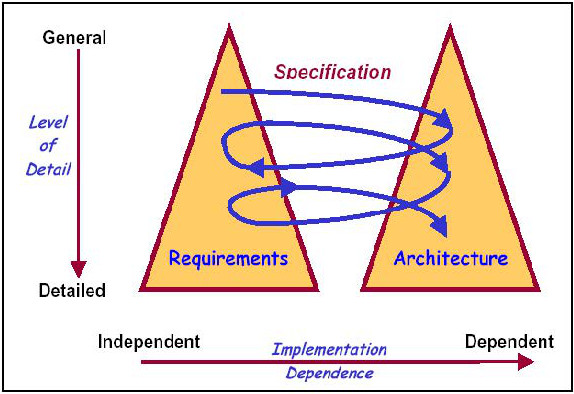
\includegraphics[width=0.7\linewidth]{fig/anforderungsengineering}
	\caption{Zusammenhang Anforderungen und Architektur}
	\label{fig:anforderungsengineering}
\end{figure}
Das Anforderungsengineering kann mit zwei Vorgehens-Modellen durchgeführt werden. Beim ersten Modell wird das Anforderungsengineering als Projektphase durchgeführt. Dabei kann jedoch auf Anforderungs-Änderung erst spät reagiert werden und der Kunde ist nicht zufrieden. Bei Modellen wie SoDa oder Scrum werden die Anforderungen kontinuierlich (just in time) erhoben. Am Anfang eines Projektes definiert man die Anforderungen nur grob und geht zusammen mit dem Kunden immer mehr ins Detail.

\subsection{Anforderungs-Techniken}

Anforderungen könne aus verschiedenen Quellen (Stakeholder, Dokumente usw.) und mit verschiedenen Ermittlungstechniken erhoben werden. Um diese Anforderungen festzuhalten werden folgende Techniken eingesetzt:
\begin{description}
	\item[Systemkontext:] Abgrenzung des Produktumfanges (Kontextdiagramm)
	\item[Ziele:] Es werden die Intentionen der Kunden festgehalten (keine Lösungsansätze dokumentieren)
	\item[Szenarien:] exemplarische, konkrete Abläufe festhalten (z.B. in Form von Use Cases, Szenario-Beschreibungen, User-Story)
	\item[Geschäftsregeln:] Regeln für unternehmerische Entscheidungen z.B. in Form von Entscheidungstabellen
	\item[Lösungsorientierte Anforderungen:] Datenstrukturen, Verhalten, Funktionssicht eines Systems, Schnittstellenbeschreibungen usw.
\end{description}
Mit einem Kontextdiagramm wird das System und dessen Kontext klar abgegrenzt. Typische Inhalte eines Kontextes sind Personen, technische Systeme oder Prozesse. Die Systemgrenze separiert das geplante System von seiner Umgebung (Lieferumfang). Möchte man ein Kontextdiagramm erstellen muss zuerst die Systemgrenze festgelegt werden. Danach sollte überlegt werden was alles zum Kontext gehört um anschliessend die Kontextgrenze festlegen zu können. Am Schluss wird noch der Nachrichtenfluss zwischen dem System und dem Kontext über Schnittstellen festgelegt. Es geht darum auch aufzuzeigen was nicht Teil des zu entwickelnden Systems ist (Definition des Lieferumfangs)!

\subsection{Anforderungen mit Use Cases festhalten}

Use Cases sind eine Technik um Anforderungen festzuhalten. In einem Use Case wird textuell eine Sequenz von Interaktion zwischen dem Benutzer und dem System beschrieben (als Text oder als Flussdiagramm). Dieser Ablauf sollte dem Benutzer einen Nutzen bringen. Auch allfällige Sonderfälle werden beschrieben. Use Cases können überarbeitet und verfeinert werden z.B. durch Pre-/Post-Condition, alternative flows oder nichtfunktionale Anforderungen. Use Cases eignen sich gut um mit dem Kunden wichtige Abläufe durchzugehen.

Sämtliche Use Cases und Benutzer eines Systems werden in einem Use Case Diagramm zusammengefasst. Mit Pfeilen kann festgelegt werden ob ein Benutzer einen Use Case auslöst oder von einem Use Case benötigt wird. Abbildung \ref{fig:use-case-diagramm} zeigt ein Use Case Diagramm.
\begin{figure}
\centering
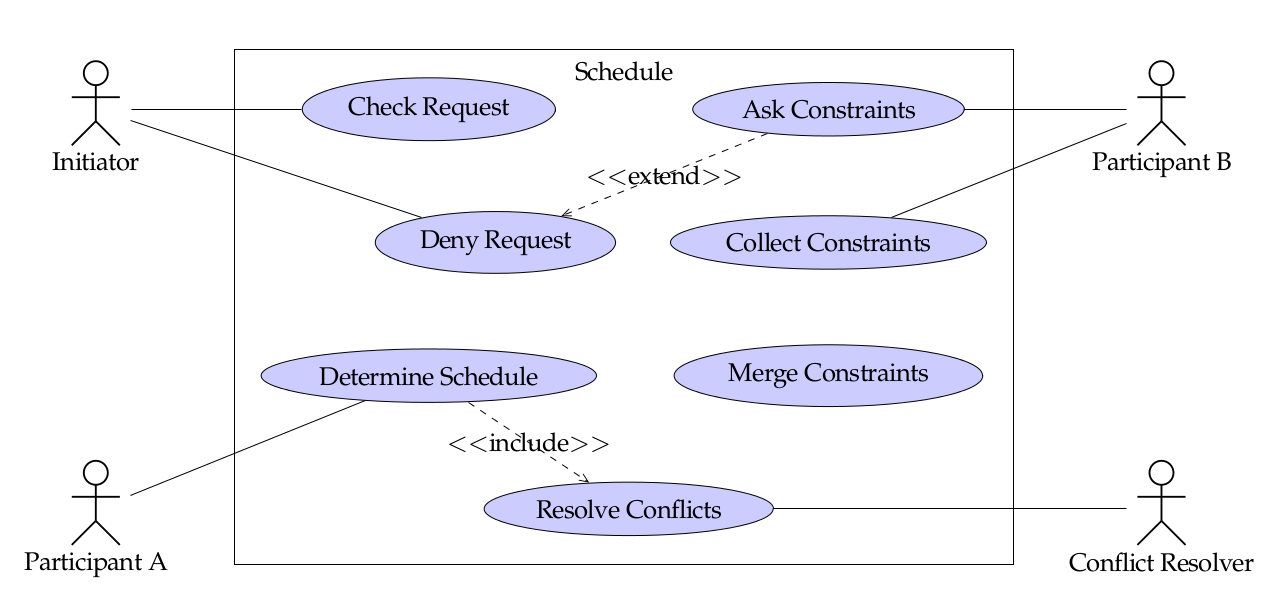
\includegraphics[width=\linewidth]{fig/use-case-diagramm}
\caption{Use Case Diagramm}
\label{fig:use-case-diagramm}
\end{figure}

\subsection{Anforderungen textuell festhalten}

Alternativ zu den Use Cases können Anforderungen auch rein textuell festgehalten werden. Eine Möglichkeit wäre die Feature-Liste. Dabei werden alle Anforderungen in einer Tabelle festgehalten und evtl. mit Priorität, Aufwand oder Risiko ergänzt. Die Features können auch detailliert werden und in Unter-Feature zerlegt werden. Eine weitere Möglichkeit Anforderungen textuell festzuhalten sind User Stories wie sie in Scrum verwendet werden. User Stories werden aus Benutzersicht geschrieben und haben immer folgendes Format:
\begin{quote}
	As a \emph{user role}, I need a \emph{functionality}, so that I get \emph{business value}
\end{quote}
Zu jeder User Story gehören Akzeptanzkriterien um die Vollständigkeit zu garantieren. Gute User Stories sind INVEST:
\begin{tabbing}
	\hspace{3cm}\=\kill
	\textbf{I}ndependent: \> möglichst unabhängig voneinander \\
	\textbf{N}egotiable: \> zerlegbar, komponierbar, änderbar, verhandelbar \\
	\textbf{V}aluable: \> hat wirtschaftlichen Wert \\
	\textbf{E}stimatable: \> so klar, dass es vom Team geschätzt werden kann \\
	\textbf{S}mall: \> klein genug, um in einem Sprint entwickelt werden zu können \\
	\textbf{T}estable: \> klare Akzeptanzkriterien 
\end{tabbing}
User Stories lassen sich auf drei Arten zerlegen (detaillieren):
\begin{enumerate}
	\item Nach Daten
	\item Nach Benutzer/Rollen
	\item Nach Prozessschritten
\end{enumerate}

\subsection{Anforderungen mit Modellen festhalten}

Anforderungen lassen sich auch mit Modellen darstellen. Durch eine objektorientierte Analyse (OOA) lässt sich ein Fach- oder Domänenmodell erstellen. Dieses Modell beschreibt das Anwendungsgebiet (Domäne) der Software in der Sprache des Benutzers und fokusiert sich dabei auf die Fachobjekte (Entitäten). Dargestellt wird es beispielsweise in UML oder wie in Abbildung \ref{fig:komisches-modell-ohne-namen}.
\begin{figure}
	\centering
	\begin{subfigure}[b]{0.4\textwidth}
		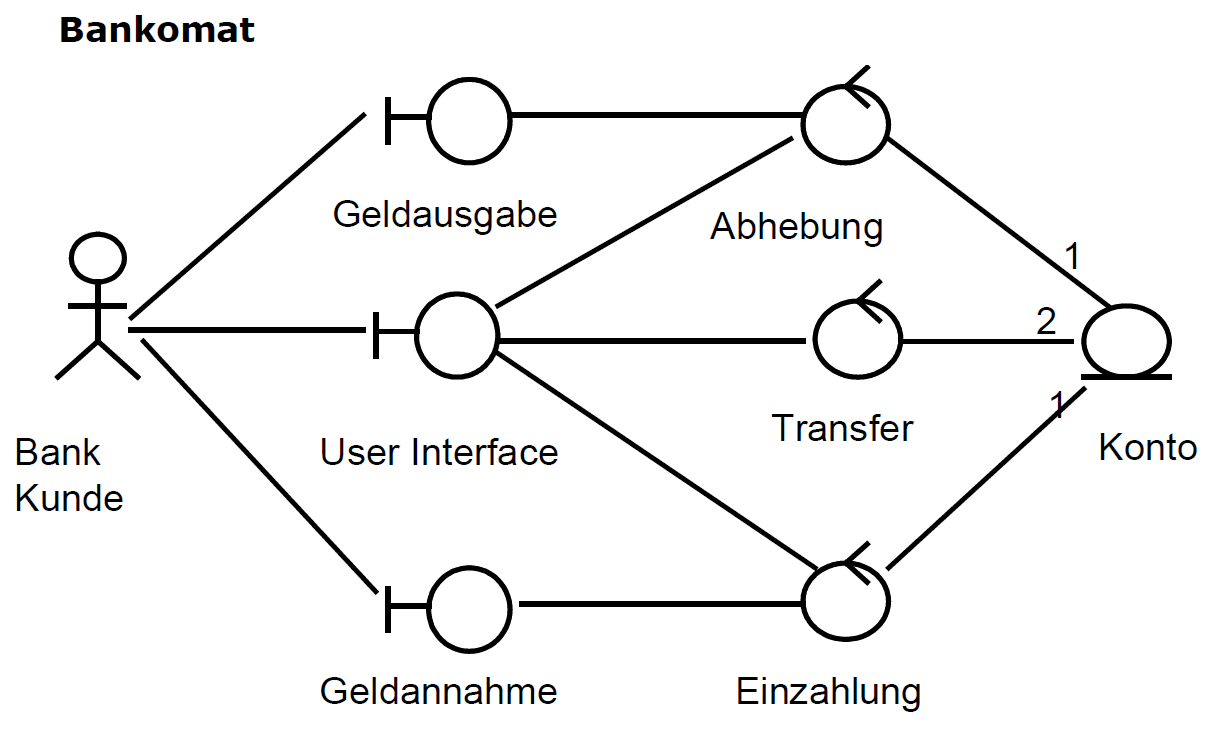
\includegraphics[width=\linewidth]{fig/komisches-modell-ohne-namen-1}
	\end{subfigure}
	\begin{subfigure}[b]{0.5\textwidth}
		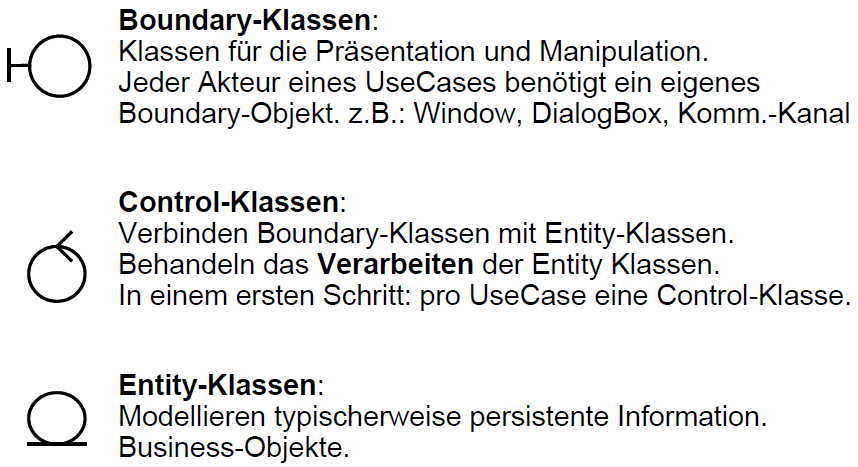
\includegraphics[width=\linewidth]{fig/komisches-modell-ohne-namen-2}
	\end{subfigure}
	\caption{Komisches Modell ohne Namen}
	\label{fig:komisches-modell-ohne-namen}
\end{figure}
Für dynamische Anforderungen können Sequenzdiagramme verwendet werden. Diese Modelle beschreiben Anforderungen und keine Lösungen.

\subsection{Prototypen}

Prototypen werden zu verschiedenen Zwecken erstellt:
\begin{itemize}
	\item Experimenteller Prototyp: zur Beurteilung bestimmter Problemlösungen. Ziel ist es nachzuweisen, dass Spezifikationen oder Ideen tauglich sind.
	\item Prototyp als Teil der Produkt-Definition (GUI-Protoyp).
	\item Evolutionäres Prototyping: Der Prototyp ist funktionsfähig und wird bis zur Produktreife weiterentwickelt (Scrum). 
\end{itemize}
Es gibt zwei Typen von Prototypen:
\begin{description}
	\item[Vertikale Prototypen:] Es werden nur bestimmte Funktionen über alle Layers getestet (Machbarkeit)
	\item[Horizontale Prototypen:] Es wird nur von einem Layer ein Prototyp erstellt (z.B. GUI)
\end{description}
Durch Prototypen ergeben sich folgende Vor-/Nachteile:
\begin{itemize}
	\item[+] Reduktion der Entwicklungsrisiken
	\item[+] Kreativität, neue Lösungsansätze
	\item[+] GUI-Prototyp: Ideal für die Diskussion mit Kunde
	\item[--] Kosten
	\item[--] Illusion nach Aussen: Projekt bereits fertig
\end{itemize}

\subsection{Dokumentation von Anforderungen}

Da Anforderungsdokumente als Grundlage für die Projektplanung, Kostenschätzung, Implementierung, Testen usw. dienen, müssen sie gewissen Qualitätskriterien erfüllen. Diese Kriterien sind nachfolgend aufgelistet:
\begin{itemize}
	\item Eindeutigkeit und Konsistenz
	\item Klare Struktur
	\item Erweiterbarkeit
	\item Vollständigkeit
	\item Verfolgbarkeit (Traceability) der Beziehungen unterschiedlicher Dokumente (inkl. Code)
\end{itemize}
Um diese Kriterien zu erfüllen wurden verschiedene Normen und Empfehlungen erstellt. Bei der DIN-Norm wird vom Kunden ein Lastenheft und vom Lieferant ein Pflichtenheft verlangt. Auch das IEEE stellt mit der SRS 830 eine Dokumentenvorlage für Anforderungen zur Verfügung.

\subsection{Anforderungen verwalten}

Um Anforderungen besser verwalten zu können sollten folgende Punkte beachtet werden:
\begin{itemize}
	\item Priorisierung
	\item Verfolgbarkeit (Traceability), die Fähigkeit eine Anforderung über den gesamten Lebenszyklus des Systems hinweg zu verfolgen (Dokumente und Code)
	\item Verwaltung von Anforderungsänderungen
	\item Anforderungen mit Attributen versehen (ID, Name, Beschreibung, Version, Autor, Quelle, Priorität, Kritikalität) 
\end{itemize}

\subsection{Use Case vs. User Story}
Ersetzt das eine das andere? Nein. Es sind zwei unterschiedliche Dinge. Use Case werden detailliert beschrieben und sind eher schwergewichtige Dokumentationsinstrumente wohingegen User Story eher zur Besprechung dienen und auch als leichtgewichtige Planungsinstrumente dienen. Prominente Methodiker wie Martin Fowler gehen davon aus, dass es zwei verschiedene Instrumente sind, welche sich ergänzen können. Quelle: http://blog.hood-group.com/blog/2013/05/15/use-cases-und-user-stories-verbundete-oder-feinde/

\section{Planung}

\subsection{Rahmenplan}

Der Rahmenplan wird in der Initialisierungsphase erstellt und die Meilensteine definiert. Ein grosses Risiko in einem Projekt stellen neue Technologien dar. Deshalb sollten diese möglichst früh mit einem Prototypen überprüft werden

\begin{figure}[h!]
\centering
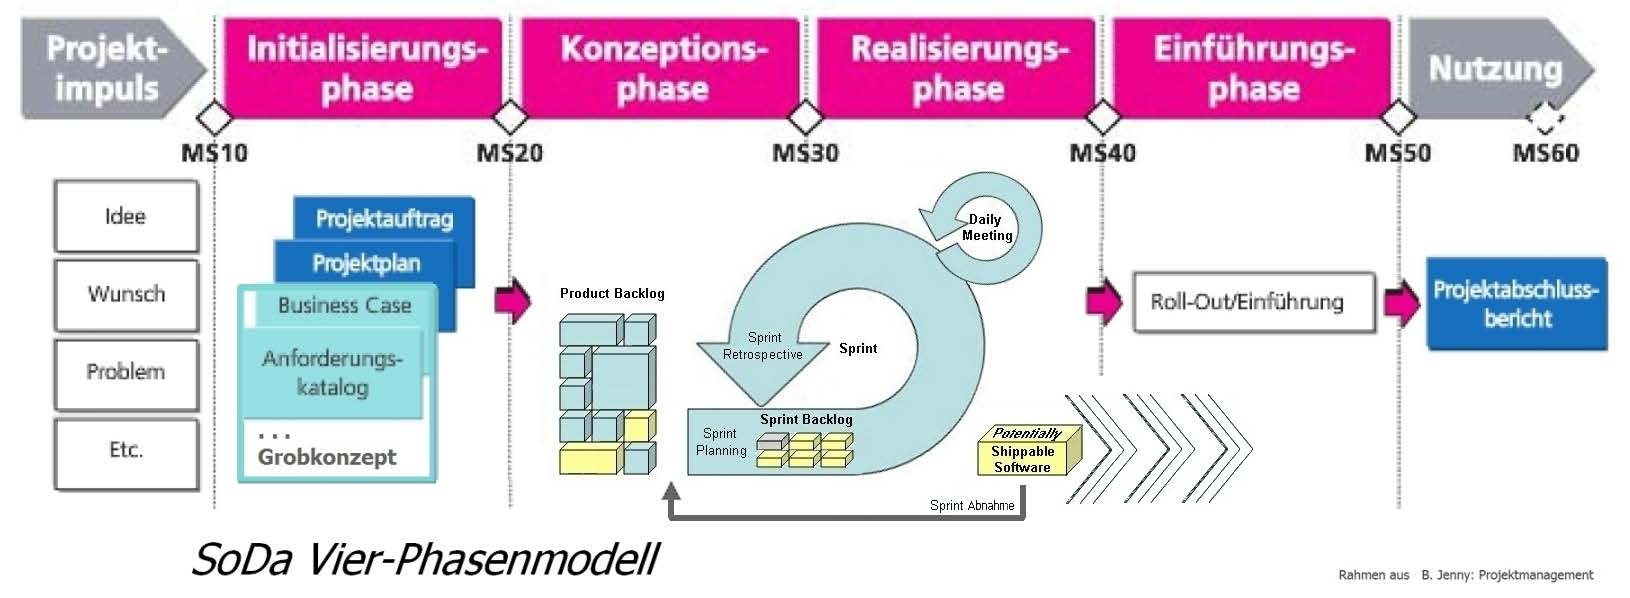
\includegraphics[width=0.8\linewidth]{fig/rahmenplan}
\caption{Rahmenplan SODA}
\label{fig:rahmenplan}
\end{figure}

Ein Meilenstein ist eine Verknüpfung von messbaren Ergebnissen zu einem definierten Zeitpunkt. Meilensteine dienen der Überwachung des Projektes und dem Einleiten von notwendigen Massnahmen. Wird folglich ein Meilenstein nicht erreicht muss man sich über einen Projektabbruch Gedanken machen.

\subsection{Scrum}

Der Inhalt eines Sprints plant man definitiv bevor man den Sprint beginnt. Der übernächste Sprint wird grob geplant. Ein Sprint enthält typischerweise drei bis sechs Userstories. Das Resultat eine Sprints muss ein \emph{potentially shippable product} sein. Das heisst die Software entspricht den Anforderungen und ist getestet. Zudem ist die Software integriert und funktioniert auf einer realitätsnahen Umgebung. Stories sollten primär neue Funktionen beschreiben. Unterstützungstätigkeiten (Konzepte, Tests, Dokumente usw.) sollten als Tasks innerhalb der Stories definiert werden.

Der Product Owner ist verantwortlich für das Produkt. Er ist die Schnittstelle zum Kunden und erstellt aufgrund dessen die Anforderungen. Da er auch für den wirtschaftlichen Erfolg des Produktes verantwortlich ist, misst er den Projektfortschritt und führt die Akzeptanztests durch. Zudem priorisiert er die Anforderungen aus dem Backlog und definiert mit dem Team die Sprintinhalte.

Der Product Backlog ist eine geordnete Liste mit allem, was in dem Produkt benötigt werden könnte. Er ist die einzige Quelle für Anforderungen. Er enthält zudem unkritische Bugs (kritische in Sprint Backlog) und Spikes (Forschungsaufträge). Ein guter Backlog ist \textbf{DEEP}:
\begin{itemize}
	\item \textbf{D}etailed Apropriately (angemessen Detailliert)
	\item \textbf{E}stimated (Geschätzt)
	\item \textbf{E}mergent (Entwickelt sich, wird gepflegt)
	\item \textbf{P}rioritized (Priorisiert)
\end{itemize}
Der Product Backlog besteht aus Backlog-Items. Zu jedem Backlog-Item gehören Akzeptanzkriterien. Ein Backlog-Item kann ein Epic, eine User Story oder ein sonstiges Work Item sein (Bugs, Spikes, Doku oder Infrastruktur). Der Sprint Backlog enthält für jeden öffentlich alle Anforderungen, Tasks und kritische Fehler für den Sprint.

Ein Sprint gliedert sich in eine Sprint Planung, der Sprint Durchführung und dem Sprint Abschluss. 
Bei der Sprint Planung stellt der Product Owner das Sprint-Ziel und wichtige Anforderungen vor. Das Team wählt und schätzt die Anforderungen zusammen mit dem Product Owner. Danach plant das Team die einzelnen Task der Anforderungen. Die Planung darf jedoch nicht überhand nehmen.
Bei der Sprint Durchführung arbeitet das Team Tasks aus dem Sprint Backlog ab. Fertige Anforderungen werden zur Kontrolle auf dem Burn-Down Chart vermerkt. Der Produkt Qwner nimmt die fertigen Anforderungen ab. 
Der Sprint Abschluss wird zusätzlich noch in einen Sprint Review und einer Retrospektive unterteilt. Der Sprint Review ist eine öffentliche Veranstaltung auch für den Kunden. Die fertige Anforderungen werden vorgeführt. Bei der Retrospektive reflektiert das Team den letzten Sprint. Gutes wird beibehalten und Probleme werden behoben.

\section{Modellieren}

\chapter{Teil von Roland Gisler}

\section{Architektur}
Eine Architektur ist eine \textbf{Abstraktion} in welcher etwas zusammenfassend und vereinfacht dargestellt wird. Mittels einer Architektur wird ein System beschrieben:

\begin{description}
	\item[Struktur und Aufbau] werden durch Elemente wie Sub- und Teilsystemen dargestellt.
	\item[Softwareteile] werden mittels Aufgaben, Zuständigkeiten und Komponenten beschrieben.
	\item [Beziehungen] untereinander werden mit Abhängigkeiten, Schnittstellen und Datenflüsse modelliert.
\end{description}

Das schlimmste Gift einer Architektur sind zyklische Abhängigkeiten. Die am häufigst verwendete Schnittstelle ist die File-Schnittstelle (Grund: Robust).

\subsection{Aspekte der Architektur}
\begin{description}
	\item[Grundlegende Struktur:] Schichten, Client/Server, n-tiers, Architekturmuster
	\item[Kommunikation und Verarbeitung:] Kommunikationsmuster (Synchron/Asynchron), Verteilbarkeit, Parallelität, Performance, Robustheit
	\item[Technologien:] Userinterface (Fat-, Rich- oder Thin-Client), Persistenz der Daten (Frameworks, O/R-Mapping), Referenzarchitekturen
	\item[Qualitätsaspekte:] Wartungsfreundlichkeit, Erweiterbarkeit
\end{description}

\subsection{System und Subsystem}
Ein System ist die Gesamtheit von Elementen, welche aufgaben-, sinn- oder zweckgebunden sind. Verfügt über klare Abgrenzung zu seiner Umwelt und wird organisiert durch Struktur und Beziehung.

\subsection{Softwaresysteme und Subsysteme}
Softwaresysteme werden wenn möglich immer zerlegt in einzelne Subsysteme (Teilsysteme). Zerlegung erfolgt meist mehrstufig hierarchisch. Subsysteme haben eine gewisse Unabhängigkeit und kommunizieren nur über wohldefinierte Schnittstellen miteinander. Dies ermöglicht folgende Vorteile:
\begin{itemize}
	\item präzisere Schätz- und Planbarkeit
	\item unabhängige Entwicklung möglich
	\item einfache Testbarkeit
	\item Potential für Wiederverwendung höher
	\item grössere Sicherheit
	\item höhere Stabilität und Robustheit
\end{itemize}
Diese Punkte sollten auch als Motivation gelten für eine gute Architektur. Es wird einfacher, verständlicher und übersichtlicher!

\subsection{Komponenten und (Sub-)systeme}
Eine Komponente ist eine softwaretechnische Einheit mit welcher man ein System realisieren kann. Ein System braucht nicht zwingend eine Komponente. Eine Komponente kann zur Realisation von mehreren Systemen verwendet werden. Komponente und System sind orthogonal.

\subsection{Architekturmuster}
Beschreibt als Konzept den Grundaufbau eines ganzen Systems. Wohingegen Entwurfsmuster nur Konzepte für Teilprobleme sind. Architekturmuster sind nicht so stark vereinheitlicht wie Entwurfsmuster. Architekturmuster gibt es für verschiedene Aspekte: Um komplexe Systeme zu strukturieren, für verteilte Systeme, für interaktive Systeme, usw.

\subsubsection{Logische Aufteilung}

\paragraph{Schichten} Mittels Schichten kann ein System aufbauend, funktional und getrennt gegliedert werden. Die Kommunikation erfolgt über wohldefinierte Schnittstellen. Abhängigkeit nur in Richtung der tieferliegenden Schicht. Achtung: Bei physischer Verteilung der einzelnen Schichten spricht man von \textbf{tiers}.
Schichten überspringen oder einen Call auf die falsche Seite ist eine Architekturverletzung und wird mit der höchst Strafe geahndet!

\paragraph{Schichtenbildung} Nach folgenden Kriterien können Schichten getrennt werden. Die Reihenfolge ist zur präferieren.
\begin{enumerate}
	\item Logische Schichtung
	\item Abstraktionslevel
	\item Technologie
\end{enumerate}
	
Beispiel mittels Java-Packages:
\textit{ch.domain.system.layerx, ch.domain.system.subsystem.layery}

\paragraph{Logische 3 Schichten-Architektur} Eine solche Aufteilung lohnt sich fast immer, unabhängig von der späteren physischen Verteilung.
\begin{description}
	\item[Präsentation] aka Presentation Layer, (G)UI-Layer. Visualisierung, User-Interface, UI-Logik. z.B. Bestellmaske für Artikel.
	\item[Geschäftslogik] aka Business(logic) Layer, Domain Layer. Implementation der Geschäftsprozesse und -modelle. z.B. Ablauf einer Bestellung, Modell eines Artikel.
	\item[Datenhaltung] aka Data Layer, Persistence Layer. Persistente Datenspeicherung, Datenlogik. z.B. Speicherung der Artikeldaten in einem RDBMS.
\end{description}

\paragraph{Verfeinerung Präsentationsschicht} Bei einem reinen Rich-GUI/Client ist es durchaus möglich, die reine Präsentation (Formulare, Dialoge) von der Präsentationslogik noch stärker zu trennen. Bspw. mittels MVC. Bei Thin-Clients (Web/HTML) ist die Trennung sogar zwingend notwendig. View wird durch HTML realisiert, Modelle und Präsentationslogik müssen im Server sein.

\paragraph{Verfeinerung Geschäftslogikschicht} Hier trennt man zwischen \textbf{Business Objects} und \textbf{Business Services}. Business Object (Domain Object) ist ein reines objektorientiertes Modell, unabhängig von Präsentation als auch von Persistenz, enthalten Daten und Methoden. Business Services enthält Klassen für die Geschäftsprozesse, arbeitet mit Business Objects. Bspw. der Business Service ''Bestellen'', kann technologisch noch weiter verfeinert werden. Einen Business Service als Webservice anbieten.

\paragraph{Verfeinerung Datenhaltungsschicht} Abstraktion der reinen Datenlogik. Diese ist unabhängig vom DBMS und vom physischen Datenmodell. Bspw. mittels O/R-Mapping. Transparentes Einbinden von Legacy-Systemen. Abstraktion mehrere Backend (DBMS)-Systeme.

\paragraph{Resultat dieser Verfeinerung}
Wenn man diese Verfeinerung vornimmt kommt man zu dieser 6-Schichten Architektur.
\begin{enumerate}
	\item Visualisation, User Interface: Formulare, Dialoge 
	\item User Interface Logik: Steuerung des UI, Ablauf
	\item Business Services, Business Logik: Fachliche Prozesse
	\item Business Objects, Business Modell: Fachliches Modell
	\item Datenlogik, Integrität: Fachliches Datenmodell
	\item Infrastruktur: z.B. O/R-Mapping-/Persistenzframework
\end{enumerate}
Bei mehr als 3 Schichten, spricht man in der Regeln von n-Schicht-Architektur.

Wie viele Schichten sollte ich implementieren? Es gibt keine konkrete Anzahl. Nachfolgend Vorteile für mehrere Schichten:
\begin{itemize}
	\item Bessere Strukturierung, einzelne Schichten klarer und einfacher.
	\item Grössere Chance für Wiederverwendung
	\item Höhere Flexibilität z.B. Austausch einzelner Schichten
	\item Bessere Skalierbarkeit
	\item Einfachere und präzisere Planung/Schätzbarkeit
	\item Parallele und getrennte Entwicklung möglich.
\end{itemize}

.. und Nachteile für mehrere Schichten:
\begin{itemize}
	\item Komplexität des gesamten Systems wird grösser
	\item Mehrere Schnittstellen, mehr Aufwand, mehr Planung.
\end{itemize}

\subsubsection{Physische Aufteilung}
\paragraph{Verteilte Architekturen: tiers} Schichtenbildung ist eine fundamentale Grundlage um verteilte Architekturen zu realisieren. Naheliegend eignen sich besonders die Schichtengrenzen zur Auftrennung um Teile auf verschiedene Systeme zu deployen. Wenn vorhandene Schichten auch physisch getrennt werden, spricht man von tiers. Populäre verteilte Architekturen sind: Client/Server (2-tier), Web-Anwendung (n-tier).

\paragraph{2-tier: Client/Server}
Klassisch: GUI-Client greift direkt auf DB-Server zu. Typisch kennt man n-Clients und 1-DB Server (n:1). Natürlich auch n:n möglich. Dies kennt man heute eher im firmeninternen Bereich (Intranet). Ist häufig auch plattformspezifisch. Die Datenhaltung und Integrität wird mittels Datenmodell und Constraints gewährleistet, die Datenlogik wird u.a. mittels Trigger/Procedures realisiert.

Es ist eine einfache Architektur und gut überblickbar. Die Datenhaltung ist zentral. Jedoch für grosse / komplexe Anwendungen gibt es keinen guten Ort für die Business-Logik. Der Client wird fat, Bussiness-Logik ist redundant vorhanden, Änderungen verlangen vollständiges redeployment. Falls im DB-Server programmiert wird, dann gibt es x unterschiedlche Sprachen je nach DMS-Hersteller. Hohe Last durch Prozeduren, Triggers und co. Wenn man einen Teil im Client und einem Teil im DB Server implementiert, dann ist es oft schwierig zu sagen, was nun wo hin soll. Demzufolge auch schlechte Wartbarkeit, weniger elegant.

\paragraph{3-tier Architektur}
Basis für die meisten Enterprise Architekturen. Typisch m:1:n (Client:Business-Daten).

Keine Redundanz der Logik vorhanden. Potential: Einbinden mehrere verschiedener Datenquellen. Verschiedene Clients realisierbar (Technologie, Umfang, Fachlich). Echte Zentralisierung von reiner Business-Logik möglich. Clients können ''rich'' sein, sind aber nicht ''fat''.

Die Aufteilung ermöglicht einen effizientere Nutzung der vorhandenen Rechenleistung. Bzw. Clients können redimensioniert werden. Falls das Design aber schlecht ist, dann kann die Kommunikation zwischen den verteilten Tiers kritisch werden. Potentiell hoher Ressourcenbedarf (Speicher) im Middle-Tier.

\subsection{MVC}
Dies ist ein Designmuster mit dem Ziel Datemodell von seiner Darstellung und deren Steuerung strikte zu trennen. Wichtig: Die exakte Implementation variiert nach Anwendungsfall und Programmiersprache! Es ist weder ein Design Pattern noch ein Architekturmuster. Es ist ein Zwitter!

\paragraph{Anwendungsfall 1: MVC in GUI-Widgets wie Swing} Controller und View sind oft zusammengefasst. Das Model existiert jedoch autonom.

\paragraph{Anwendungsfall 2: MVC auf Applikationsebene} Model ist meist eine ganz normale Java-Klasse. Mehrere Views können die Daten darstellen. Änderungen im Modell werden an die Views gesendet. Modell darf aber View nicht kennen (Observer)! Ein Controller verändert die Modelle und ordnet den Views die entsprechenden Modelle zu. Bsp: Modell einer Kundenadresse. Zwei Views: Detailliertes Formulare und als Zeile in Tabellenansicht.

\begin{figure}[h!]
	\centering
	\begin{subfigure}[b]{0.3\textwidth}
		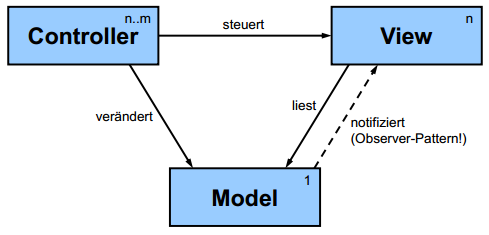
\includegraphics[width=\textwidth]{fig/mvc}
		\caption{MVC Prinzip}
		\label{fig:mvc}
	\end{subfigure}
	~
	\begin{subfigure}[b]{0.3\textwidth}
		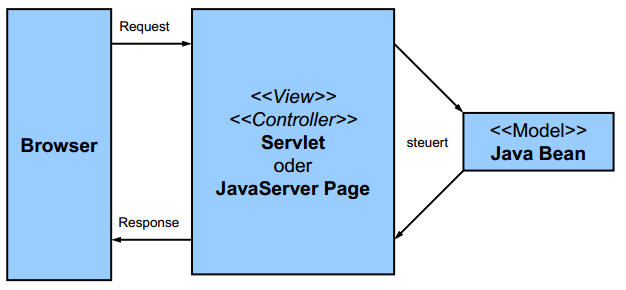
\includegraphics[width=\textwidth]{fig/mvc-web-1}
		\caption{MVC Variante 1: Alt und eher schlecht. (View Controller vermischt)}
		\label{fig:mvc-web-1}
	\end{subfigure}
	~
	\begin{subfigure}[b]{0.3\textwidth}
		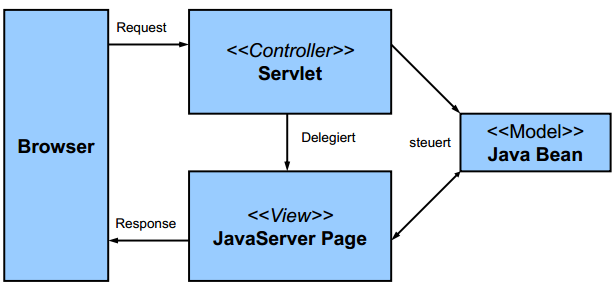
\includegraphics[width=\textwidth]{fig/mvc-web-2}
		\caption{MVC Variante 2: Neu und eher besser.}
		\label{fig:mvc-web-2}
	\end{subfigure}
	\caption{MVC Pattern}\label{fig:mvc-pattern}
\end{figure}

\paragraph{Implementationsvarianten} Kopplung zwischen Model und View. Observerpattern zwischen Modell und View oder über Controller. Statisches Modell: Notifikation über Änderungen im Modell (eher bei grösseren Modellen mit wenig Änderungen). Dynamisches Modell: Aktuelles Modell wird der View regelmässig übergeben (eher bei kleineren Modellen mit vielen Änderungen).

\paragraph{MVC in Webapplikationen} 
MVC Architektur ist bedingt durch die Technologie von Web-Applikationen eine Herauserforderung. Es besteht oft die Gefahr View und Business-Logic zu vermischen. Modell kann jeweils relativ einfach extrahiert werden. Im Laufe der Zeit sind zwei MVC-Varianten entstanden:

MVC Pattern ist fundamental im SW-Design. Modelle sind meist sehr stabil und bieten hohe Kohäsion und lose Kopplung. Pro Modell können verschiedene Views existieren. Die Wiederverwendung von Controller ist jedoch sehr gering, da oft hoch spezialisiert. Controller agieren als Leim zwischen View und Modell.

\paragraph{Alternativen} Es gibt weitere Varianten wie MVP von IBM, Taligent, Martin Fowler. Grundsätzlich will man View unabhängiger vom Modell gestalten. Mehr Potential beim Testen!

\subsection{Implementation der Business Logik}
Es muss wie immer gut wartbar und erweiterbar sein, hohe Wiederverwendung haben. Einfache Integration verschiedener Technologien, möglichst hohe Technologieunabhängigkeit.

\subsubsection{Domain Logic Pattern: Transaction Script}
Strukturiert Geschäftslogik in einzelne in sich abgeschlossene Funktionen. Transaktion im Sinne von ''logical unit of work''.

Klassisches EVA-Prinzip. Alte Idee mit Ursprung in Hostsystemen mit Terminals (Host-Transaktionen). Sehr starke Kopplung zu Präsentation und Datenbank. Hohe Spezialisierung, schlechte Austauschbarkeit. Gute Performance, weil minimaler Overhead. Für kleine Systeme, einfach und schnelle Implementation. Für grosse - schlechte wartbarkeit, viel Redundanz, keine Wiederverwendung -> Nein!

\subsubsection{Domain Logic Pattern: Table Module}
Pro Entität (Tabelle) eine Klasse, welche die Businesslogik für alle Tupel enthält. Arbeitet so effizient mit ganzen Tupelmengen. Direkte Datenweitergaben an Präsentation möglich. Logisches Beispiel: Singleton Klasse Artikel mit CRUD-Operationen. Technisches Beispiel: Java Klasse, welche mit ResultSet arbeitet.

Hat den Ursprung in der zwei Schichten Architektur. Sehr starke Kopplung an DB. Für Systeme mit wenig oder einfacher Businesslogik. Für grosse Systeme ungeeignet. Für Businessprozesse, welche mehrere Entitäten betreffen drohen Redundanzen und mit grossen Datenmengen kann es kollabieren.

\subsubsection{Domain Logic Pattern: Domain Model}
Abstraktion der Geschäftsprozesse und Geschäftsdaten. Reines objektorientiertes Modell der Domäne. Vollständige Trennung von der physischen Datenspeicherung. Interaktion zwischen den Objekten. Logisches Beispiel: \textbf{Artikel} beschreibt einen konkreten Artikel, welches einem Lager zugeordnet ist. \textbf{Lager} beschreibt ein Lager in welchem Artikel sind. Hat die Fähigkeit zu reservieren, zu beziehen usw.
Technisches Beispiel: EJBs oder DomainModel mit POJOs.

Realisiert praktisch alle Vorteile einer logischen 3-Schichten Architektur. Entkopplung von der Präsentation und Datenspeicherung, hohe Wiederverwendung, gute Wart- und Erweiterbarkeit. Starke Strukturen, leichtes Verständnis. Skaliert auch für sehr grosse und komplexe Enterprise Systeme.
O/R-Mapping verursacht jedoch einen gewissen Overhead. Effizienter Datenaustausch zwischen Schichten ist eine Herauserforderung.

\subsubsection{Domain Logic Pattern: Service Layer}
Optimale Ergänzung zu einem beliebigen Domain Logic Pattern. Verschiedene Clients benötigen sehr unterschiedliche Schnittstellen.

\begin{itemize}
	\item Interaktive Anwendung (GUI)
	\item Batchorientierte Verarbeitung
	\item Datenimport / -export / Synchronisierung
\end{itemize}

Lösung: Man bietet übergeordnete Services an, welche die Businesslogik erneut kapseln. Grundlage eines Service Oriented Architecture (SOA) und eines Enterprise Service Bus (ESB). Technisches Beispiel: Webservice (Wrappen bestehende Businessfunktionalitäten)

\subsubsection{Auswahl des geeigneten Patterns}
Es kommt auf die Grösse und Komplexität des gesamten Systems an. Weitere wichtigte Aspekte sind Lebensdauer, einzelne Geschäftsprozesse.

Domain Model Pattern lohnt sich um so mehr, je grösser das System ist.

Entscheide werden oft kontrovers diskutiert. Am Besten immer problemorientiert und nicht technologieorientiert Denken. Erfahrungen sind jedoch notwendig.

\subsubsection{Distribution Patterns}
Wie werden Daten effizient zwischen den Tiers übertragen?

\begin{description}
	\item[Attributebene] Client frägt nach jedem Attribut einzel. Sehr ineffizient, viele Kommunikationsschritte.
	\item[Objektebene] Client erhält ganze Businessobjekte. Ineffizient, zu grosse Datenmengen.
\end{description}

Dieses Problem kann mit zwei Patterns angegangen werden.

\paragraph{Pattern 1: Data Transfer Objects (DTOs)} Man definiert für den Daten-Transport für unterschiedliche Services optimierte, reine Datenobjekte. Enthalten nur Daten, keine Methoden. Enthalten nur Daten, welche vom Service benötigt werden. Vorteile - nur ein Funktionsaufruf (Kommunikation) notwendig. Effizient bezüglich Datenmenge. Aber es braucht eventuell sehr viele verschiedene DTOs. Mapping notwendig: DTOs müssen erzeugt werden. DTOs sind nicht wirklich objektorientiert.

\paragraph{Pattern 2: Remote Facade} Fassadenklasse, welche die feingranularen Methodenaufrufe auf verschiedene Businessobjekte kapselt und aus den Resultaten DTOs baut. Fassade darf keine Businesslogik enthalten, Fassade übernimmt Mapping. Dies birgt den Vorteil, dass die Verbindung zwischen dem reinen objektorientierten Businessmodell und effizienter Kommunikation. Gefahr, dass man Businesslogik implementiert und ist nur ein Durchlauferhitzer.

\paragraph{Einsatz der Patterns}
Werden oft in Kombination eingesetzt. Achtung: Verwaltung der DTOs kann aufwendig werden. Model Driven Architecture kann hier helfen: Schnittstellen mit DTOs einzeln modellieren. Grosse Teile des Quellcodes auf Basis des Modells generieren. Das Mapping wird mittels Hilfswerkezug realisiert.

\subsection{Diskussion: Thin-, Richt-, Fat-Client}
Ein Thin-Client enthält nur die Präsentationsschicht. Eine HTML-Seite ist quasi ein Thin-Clien.t
Der Rich-Client ist beispielsweise ein Java-Programm, welcher aber in einer n-Tier Architektur steckt. Auf dem Client ist nur die Präsentation geregelt. Die Business-Logik befindet sich auf einem andern tier. Der Fat-Client ist die Variante einer 2-Tier-Architektur. Business Logik steckt im Client.

\subsection{Was ist oben was ist unten}
Man spricht von oben, dem GUI, und von unten, den Daten.


\section{Testing}

\subsection{Ziele für gute Tests}

Durch das Erstellen von Testcode wird die Softwarequalität nachweislich gesteigert. Damit bei Regresstests Zeit gespart werden kann sollte die Testausführung so weit als möglich automatisiert werden. Die Testfälle sollten möglichst früh im Projekt mithilfe der Use Cases erstellt werden. Zudem sollte man die Testfälle möglichst kurz und einfach halten. Dadurch werden die Testfälle stabiler gegen Veränderungen und defekte lassen sich schneller lokalisieren. Als Basis sollten die normalen Abläufe getestet werden aber auch absichtlich provozierte Fehler und nicht erlaubte Vorgänge sollen ebenfalls getestet werden. Folgendes Ziel sollte immer vor Augen gehalten werden:
\begin{quote}
Testfälle gerade so komplex wie nötig, und so einfach wie möglich halten!
\end{quote}

\subsection{Testarten}

Neben der Unterteilung in Unit-, Integrations- und Systemtests, können Tests auch in folgende Kategorien aufgeteilt werden:
\begin{description}
	\item[Funktionale Tests:] Bei dieser Testart wird die gesamte Applikation aus der Sicht des Endbenutzers getestet. Es wird die Business- und die Applikationslogik getestet. Diese Testart ist sehr aufwendig und sollte wenn möglich automatisiert werden. 
	\item[Performance-/Stresstests:] Auf der einen Seite wird ein klassisches Profiling (Memorybedarf, Antwortzeit) durchgeführt. Es wird jedoch auch getestet wie die Anwendung bei hoher Belastung durch viele Clients reagiert (Queueing oder Zurückweisen von Anfragen).
	\item[Sicherheitstests:] Die Testart testet eine Applikation auf verschiedene Sicherheitslücken. Diese Testart ist vor allem bei Webapplikationen wichtig, um z.B. SQL-Injection zu verhindern.   
\end{description}

\subsection{Testdoubles}

Bei einer Schichten-Architektur welche Bottom-Up entwickelt wurde, besteht die Gefahr dass bei Unit-Tests alle unteren Schichten mit getestet werden. Dadurch steigt die Ausführungszeit und die Abhängigkeiten. Diese Tests sind in diesem Fall Integrationstests und nicht mehr Unit-Tests.
Um die Schichten voneinander zu entkoppeln werden Testdoubles eingesetzt. Um Testdoubles erfolgreich einzusetzen, muss ein entsprechend gutes Design nach SOLID vorliegen. Vor allem das Dependency Inversion Principle (DIP) sollte beachtet werden. Abbildung \ref{fig:test-doubles} zeigt eine Übersicht über alle Testdoubles.
\begin{figure}
\centering
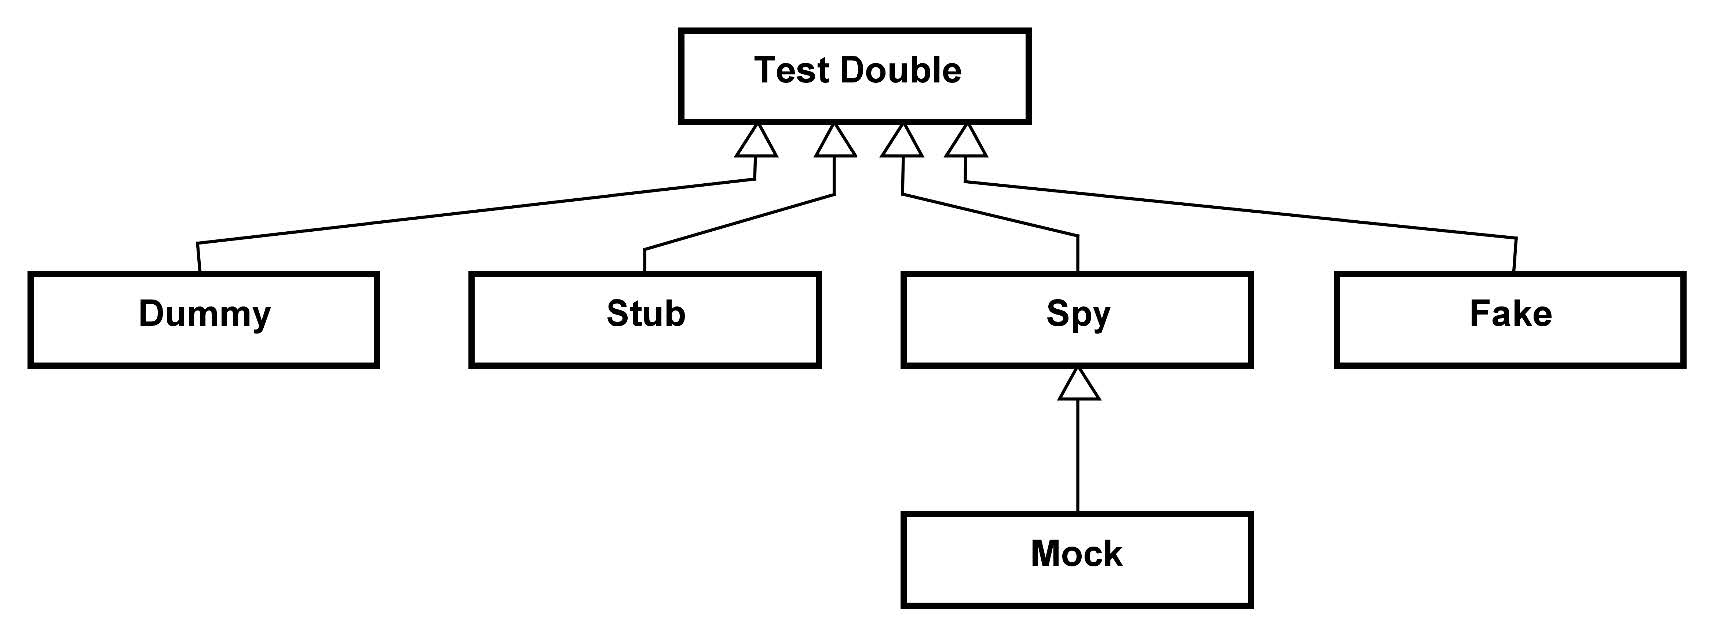
\includegraphics[width=0.7\linewidth]{fig/test-doubles}
\caption{Übersicht Test Doubles}
\label{fig:test-doubles}
\end{figure}
Nachfolgend werden alle Test Doubles im Detail beschrieben:
\begin{description}
	\item[Dummy:] Ein Dummy ist eine primitive (häufig leere) Ersatz-Implementation, welche als Parameter an eine Methode übergeben wird. Der Parameter muss für den Test vorhanden sein aber dessen Nutzung ist nicht relevant. Häufig geben Dummys einfach \texttt{null} zurück.
	\item[Stub:] Ein Stub liefert einen sinnvollen, vordefinierten Wert zurück. Für verschiedenen Testziele werden unterschiedliche Stub-Implementationen (z.B. für Fehlerfall) verwendet.
	\item[Spy:] Ein Spy liefert dynamisch Werte zurück und merkt sich die Methoden welche an ihm aufgerufen werden. Das erlaubt ein ''Behavior''-Testing.
	\item[Mock:] Ein Mock macht das gleiche wie der Spy, jedoch verifiziert er gleich selbst ob eine Methode aufgerufen wurde. Mocks werden typischerweise zur Laufzeit von Frameworks mit dem \emph{Proxy-Pattern} erstellt.
	\item[Fake:] Alternative Implementation, welche eine Komponente mit vernünftigem Aufwand ersetzen kann. Ein Fake ist manchmal besser als die eigentliche Implementation aber sehr aufwendig zu entwickeln.
\end{description}
Dummy und Stubs werden eingesetzt wenn man mit wenig Aufwand eine bessere Testisolation erreichen will. Die Test werden dadurch robuster. Spys und Mocks sind die Universalwaffen, werden jedoch oft zu häufig eingesetzt. Mit Mocks sollte man sparsam umgehen, weil sich sonst der Testcode zu stark an den Implementationscode koppelt. Ein Fake ist sehr aufwendig zum Entwickeln und wird praktisch nie eingesetzt.

\subsection{Testen von DB-Applikationen}

Die Herausforderung beim Testen von DB-Applikationen ist die Datenmanipulation durch die Testfälle. Damit diese Manipulationen reproduzierbar bleiben, muss der Datenbankinhalt vor und nach dem Test definiert/verifiziert werden. Um dies zu erreichen muss ein Testdatenmanagement betrieben werden. Beim Testdatenmanagement werden Testdaten pro Testfall bereitgestellt und aktiv gewartet.
Für das Testen von DB-Applikationen gibt es verschiedene Ansätze:
\begin{itemize}
	\item Initialisierung und Verifikation von Testdaten mit Frameworks (z.B. DBUnit)
	\item Verwendung von mehreren DB-Instanzen auf nur einem Server (z.B. 1 für Entwickler und 1 für Buildserver). Schwierig Schemas synchron zu halten und evtl. Konflikte bei paralleler Ausführung.
	\item Lokale Datenbank pro Entwickler, Buildserver usw. Je nachdem nicht möglich wegen Lizenzen jedoch keine Konflikte bei paralleler Ausführung.
	\item Nach den Tests ein Transaction Rollback durchführen (im Tear Down)
	\item In-Memory-Datenbank für jeden Test (langsam weil DB jedesmal aufgebaut werden muss)
\end{itemize}

\subsection{Testen von GUI-Applikationen}

Bei GUI-Applikationen stellt die GUI selber die Schnittstelle bereit. Die Interaktion mit der GUI muss demnach simuliert werden um Tests automatisiert durchführen zu können. Auch die Verifikation der Testergebnisse muss optisch erfolgen. Für das Testen von GUI-Applikationen werden zwei Ansätze verfolgt:
\begin{description}
	\item[Record \& Play:] Ein manueller Test wird aufgezeichnet, abgespielt und danach überprüft. Dies ist nicht zu empfehlen, weil die Prüfung schwierig/unsicher ist.
	\item[Frameworks:] Das GUI-Framework wird um die Testbarkeit erweitert. Diese Test müssen aufwendig programmiert werden. Es entsteht so eine starke Kopplung an die interne GUI-Struktur und man testet nie das Endresultat. Beispiele für GUI-Frameworks sind UISpec4J (Swing) oder TestFX (JavaFx).
\end{description}

\subsection{Testen von Web-Applikationen}

Web-Applikationen lassen sich aufgrund ihres strikten Request-/Response-Modell sehr gut testen, weil auf jede Anfrage eine definierte Antwort kommen muss. Stress- und Securitytests lassen sich so ebenfalls einfach automatisieren. In der Praxis wird diese Möglichkeit oft zu wenig genutzt. Es existieren aber für Java einige Frameworks:
\begin{itemize}
	\item HttpUnit
	\item HTMLUnit
	\item JWebUnit
	\item Selenium
\end{itemize}
Eine Voraussetzung für die Verwendung dieser Frameworks ist ein sauberer HTML-Code (z.B. alle Elemente mit id versehen). Diese Frameworks simulieren Browserzugriffe und analysieren die Antwort vom Server.
 
Web-Applikationen mit Web 2.0 Technologien (HTML 5, Ajax, JavaScript) sind schwieriger zu Testen. Diese Applikationen werden mit echten Browsern mit einem Test-Plugin getestet. Die Grundlage ist die Browser-Automation, wobei SeleniumHQ und Arquillian zwei Frameworks sind die das unterstützen. 

\section{SOLID}

Das SOLID-Prinzip fasst fünf wichtige Designprinzipen zusammen:
\begin{itemize}
	\item Single Responsibility Principle
	\item Open Closed Principle
	\item Liskov Substitution Principle
	\item Interface Segregation Principle
	\item Dependency Inversion Principle
\end{itemize}
Durch die Einhaltung der SOLID-Prinzipien erreicht man ein besseres Design. Besseres Design heisst konkret:
\begin{itemize}
	\item höhere Wiederverwendbarkeit
	\item leichtere Verständlichkeit / Lesbarkeit
	\item (stark) verbesserte Testbarkeit
	\item vereinfachte Wartung
	\item verbesserte Erweiterbarkeit
	\item leichteres Refactoring
\end{itemize}

\newpage

\subsection{Single Responsibility Principle}

\begin{itemize}
	\item Unix-Philosophie: «Tu nur ein Ding, genau ein Ding, das aber richtig!»
	\item Eine Klasse hat möglichst nur \textbf{eine} Zuständigkeit (siehe Listing \ref{lst:srp-interface})
	\item Eine Klasse hat somit nur \textbf{einen} Grund zur Änderung
	\item Änderungen oder Erweiterungen sollten sich auf möglichst wenige Klassen beschränken (hohe Kohäsion bleibt erhalten).
	\item Viele kleine Klassen sind besser als wenige grosse Klassen
	\item Wichtiger Nebeneffekt: Stark verbesserte Testbarkeit!
\end{itemize}

\begin{lstlisting}[caption={Schlechtes Interface nach SRP},label=lst:srp-interface]
// Zwei Aufgaben: Verbindungsaufbau und Datenübertragung
interface Modem {
	public void dial(String phoneNumber);
	public void hangup();
	public void send(char c);
	public char receive();
}
// Besser zwei Interfaces
interface Connection {
	public void dial(String phoneNumber);
	public void hangup();
}
interface Transmit {
	public void send(char c);
	public char receive();
}
\end{lstlisting}

\subsection{Open Closed Principle}

\begin{itemize}
	\item Eine Software-Entität soll offen für Erweiterungen, aber geschlossen gegenüber Modifikationen sein
	\item Mit OCP senkt man das Risiko neue Fehler einzubauen, weil man bestehenden Code nicht ändern muss
	\item Häufig über Einsatz des Strategy-Patterns (GoF) erreicht (siehe Listing \ref{lst:ocp-strategy})
\end{itemize}

\begin{lstlisting}[caption={Strategy Pattern um OCP umzusetzen},label=lst:ocp-strategy]
// Was passiert, wenn eine (oder hundert) neue Operation ergänzt werden soll?
double calc(Operation op, double arg1, double arg2) {
	double result = 0.0;
	switch (op) {
		case Addition:
			result = arg1 + arg2; break;
		case Subtraktion:
			result = arg1 - arg2; break;
		default:
			throw new IllegalArgumentException(); break;
	}
	return result;
}
// Pro neue Operation wird eine Klasse erstellt, welche das Interface Operation implementiert
interface Operation {
	double calc(double arg1, double arg2);
}
double calc(Operation op, double arg1, double arg2) {
	return op.calc(arg1, arg2);
}
\end{lstlisting}

\subsection{Liskov Substitution Principle}

\begin{itemize}
	\item Gut über den Sinn/die Korrektheit von Spezialisierungen nachdenken:
	\begin{itemize}
		\item Subtypen sollten sich so verhalten wie ihre Basistypen
		\item Meist ist Komposition der Vererbung vorzuziehen!
	\end{itemize}
	\item Verifiziere Entscheide mit folgenden Sätzen:
	 \begin{itemize}
		\item Subtyp ist ein (is-a) Basistyp (Vererbung)
		\item Subtyp verhält sich (behaves-as) wie ein Basistyp (Komposition)
	 \end{itemize}
	\item Macht die Implementation von \texttt{equals()} Schwierigkeiten, sollte man unbedingt die Vererbung hinterfragen!
	\item Tipp: Vererbung konsequent verhindern (\texttt{final}): Nur dort wo sinnvoll und vorgesehen explizites Design für Spezialisierungen (Design for inheritance or else prohibit it).
\end{itemize}

\subsection{Interface Segregation Principle}

\begin{itemize}
	\item Schnittstelle strikt von Details der Implementation trennen (Ist mit Java einfach: Wir haben Interfaces!)
	\item Schnittstellen sollen eine hohe Kohäsion haben
	\item Basisklassen sollten nichts von ihren Spezialisierungen wissen
	\item Kopplung zwischen Komponenten soll minimal sein
	\item Viele kleine (schmale) Schnittstellen sind besser als eine zu grosse (fette) Schnittstelle
	\item Population von Schnittstellen vermeiden (möglichst keine Vererbung von Schnittstellen)
\end{itemize}

\subsection{Dependency Inversion Principle}

\begin{itemize}
	\item DIP ist nicht gleich Dependency Injection!
	\item High-Level Klassen sollen nicht von Low-Level Klassen abhängig sein, sondern beide von Interfaces (siehe Abbildung \ref{fig:dip-beispiel})
	\item Interfaces sollen nicht von Details abhängig sein, sondern Details von Interfaces
	\item Isolation von Klassen vereinfacht/ermöglicht die Testbarkeit (ggf. auch mit Einsatz von Test Doubles)
	\item Auflösung von Dependencies über Dependency Injection (DI)
\end{itemize}

\begin{figure}[h!]
	\centering
	\begin{subfigure}[b]{0.8\textwidth}
		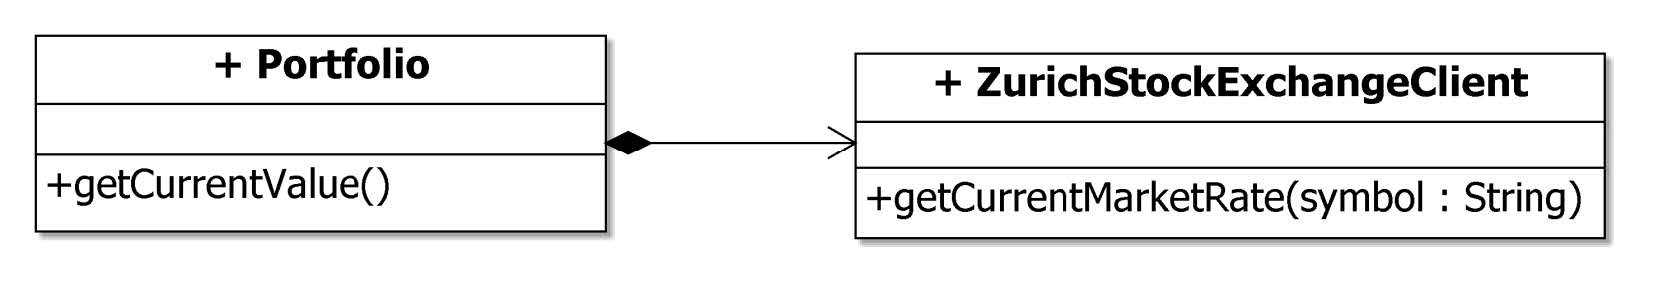
\includegraphics[width=\textwidth]{fig/dip-schlecht}
		\caption{High-Level-Klasse \texttt{Portfolio} ist abhängig von Low-Level-Klasse \texttt{ZurichStockExchangeClient} $\rightarrow$ Schlecht!}
	\end{subfigure}
	\begin{subfigure}[b]{\textwidth}
		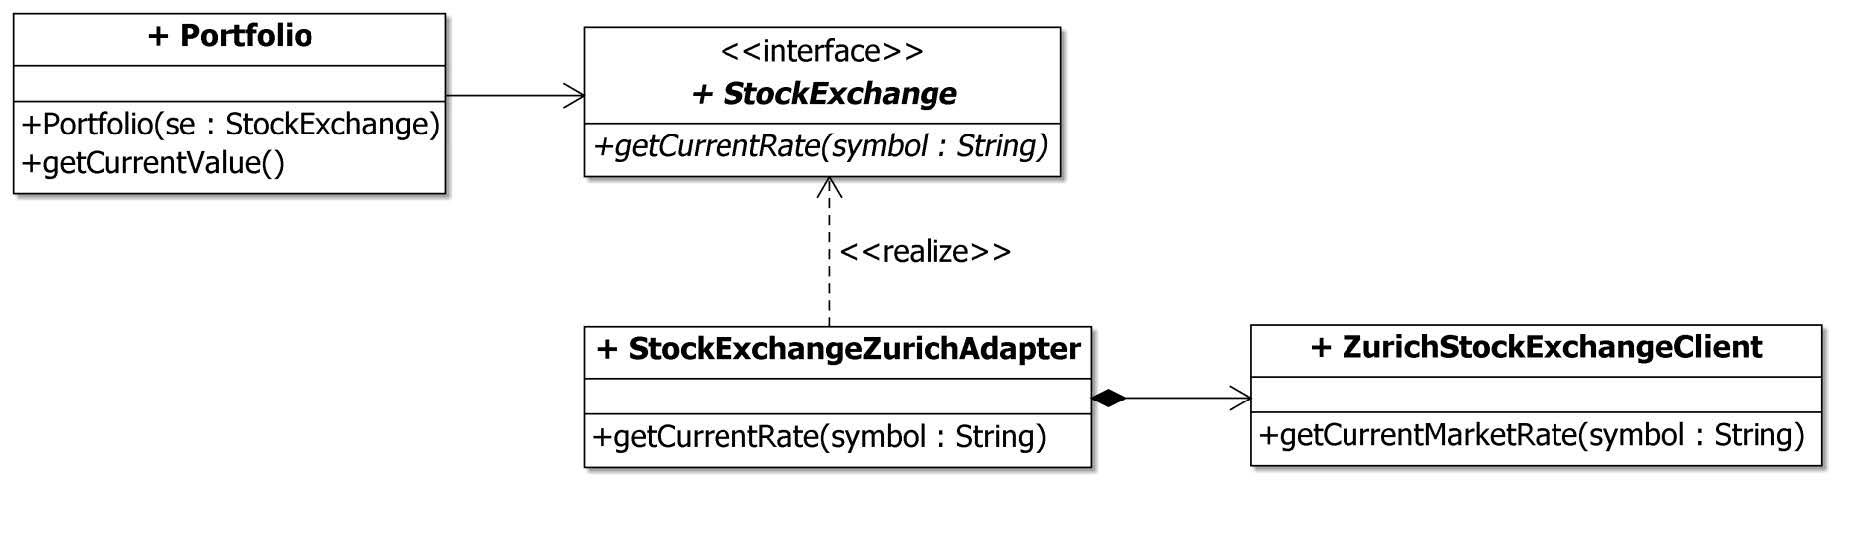
\includegraphics[width=\textwidth]{fig/dip-besser}
		\caption{Bessere Lösung: \texttt{Portfolio} unabhängig von Implementationsdetails}
	\end{subfigure}
	\caption{Beispiel DIP}\label{fig:dip-beispiel}
\end{figure}


\chapter{Teil von Prof. Dr. Ass. Roland Christen aka Surfer Boy}

\section{Persistenz}
Persistenz stammt aus dem lateinischen \emph{persistere} und steht für das langfristige Fortbestehen einer Sache. In der Informatik wollen wir das Fortbestehen der Daten sichern.

\subsection{Modellierung}
Die Datenmodellierung erfolgt auf drei Ebenen. Konzeption, Implementation und physischer Entwurf. In DMG haben wir den konzeptionellen Entwurf mittels ERM gemacht. In APPE lernen wir, dass dieser nicht Praxis tauglich ist und verwenden nun UML-Klassendiagramme (siehe Abbildung \ref{fig:konzeptionelles-datenmodell-mit-klassendiagram}).

\begin{figure}[h!]
\centering
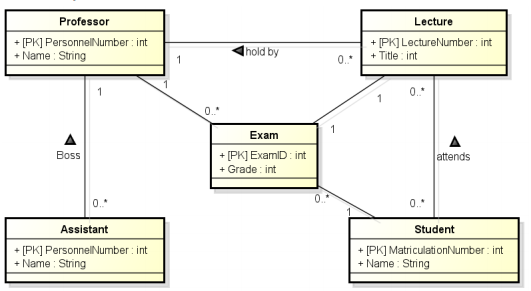
\includegraphics[width=0.7\linewidth]{fig/konzeptionelles-datenmodell-mit-klassendiagram}
\caption{Konzeptionelles Datenmodell mit UML Klassendiagrammen}
\label{fig:konzeptionelles-datenmodell-mit-klassendiagram}
\end{figure}

Nach der Konzeption folgt die Implementation. Der konzeptionelle Entwurf ist vollständig unabhängig von der konkreten Datenbank. Nun kann das konzeptionelle Modell für eine konkrete Datenbank transformiert werden. Bisher wählten wir immer relationale Datenbanken.
Ein Beispiel dafür sehen wir in Abbildung \ref{fig:relationales-datenmodell}.

\begin{figure}[h!]
\centering
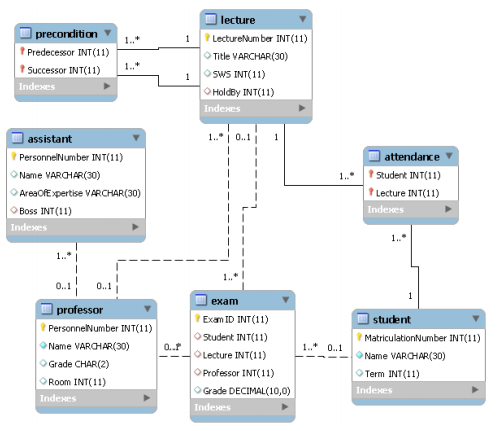
\includegraphics[width=0.7\linewidth]{fig/relationales-datenmodell}
\caption{Relationales Datenmodell}
\label{fig:relationales-datenmodell}
\end{figure}

\subsection{JPA (Java Persistence API)}
Nun haben wir das effektive Schema, welches wir auf unserem DBMS installieren können. Nun wollen wir auf die Daten aus einem Java-Programm zugreifen.

Und hier müssen wir ein ORM durchführen. ORM steht für objekt-relationales Mapping. Darauf ist die Informatik nicht stolz und es gilt als notwendiges Übel. Eine ORM Architektur ist in der Abbildung \ref{fig:orm-basics} ersichtlich.

\begin{figure}[h!]
\centering
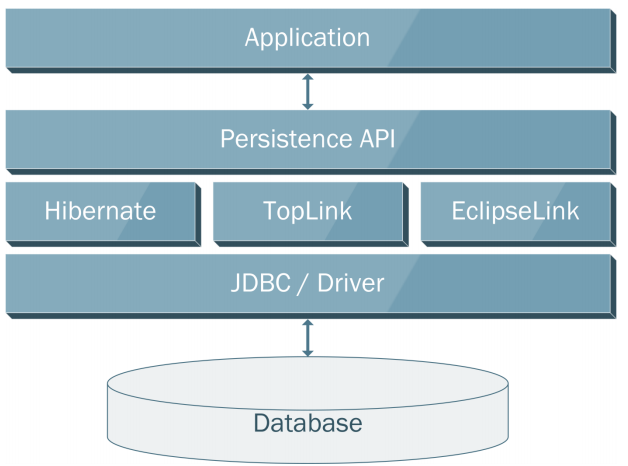
\includegraphics[width=0.7\linewidth]{fig/orm-basics}
\caption[ORM Basics]{}
\caption{}
\label{fig:orm-basics}
\end{figure}

Folgendes sind Schlüsselelemente in JPA:
\begin{itemize}
	\item Entity: Java-Klasse, welche für eine Tabelle steht.
	\item Annotation: Definitionen für das OR Mapping. Man kann auch das gesammte Mapping in XML Files definieren, aber eher Old-School und nicht fresh Surfer-like.
	\item EntityManager: Klasse um auf die Entities zuzugreifen.
	\item Persistence Unit: Konfiguration für DB-Verbindung, DB Treiber und weiteres.
	\item JPQL: Java Persistence Query Language. Objektorienterte Abfragesprache. Abstrahiert SQL vollumfänglich!
\end{itemize}

\subsubsection{Vorgehen}
Entweder macht man die Datenbank zuerst und generiert die Entities daraus. Oder man implementiert die Entities und generiert das DDL. Christens Approach ist, dass man das DDL selber schreibt und die Entities daraus generiert. Wir gehen auch so vor. Es ist extrem wichtig, dass das Datenmodell korrekt ist und wir wollen hier uns nicht auf irgendwelche Tools verlassen. Ich will genau definieren wie die Zusammenhänge sind. Ausserdem will ich Herr sein über die Attribute in welcher Domäne mit welcher Konfiguration sie stecken. Anschliessend kann man die Entities generieren - man muss sich das Mapping danach nochmals anschauen!
Um die bestimmten Objekte zu generieren, gibt es verschiedene Tools. Die IDEs wie Eclipse oder Netbeans besitzen solche Tools.

\subsubsection{Coding}
Hier ein Beispiel wie man das JPA verwendet siehe Abbildung \ref{fig:sample-jpa-code}. Die EntityManagerFactory ist teuer und sollte pro Run nur einmal instanziiert werden. Der EntityManager (not threadsafe), welcher man daraus holen kann ist leichtgewichtig und kann quasi pro Request erzeugt und wieder verworfen werden. P.S: Das ist genau das was in JavaEE passiert. Der EntityManager wird injected und zwar pro Request. Die EntityManagerFactory wird bei Applikationsstart erzeugt. Im Beispiel sehen wir auch, dass die Transaktionen manuell gestartet und geschlossen werden. In JavaEE wird das in der Regel vom Container übernommen. 

\begin{figure}[h!]
\centering
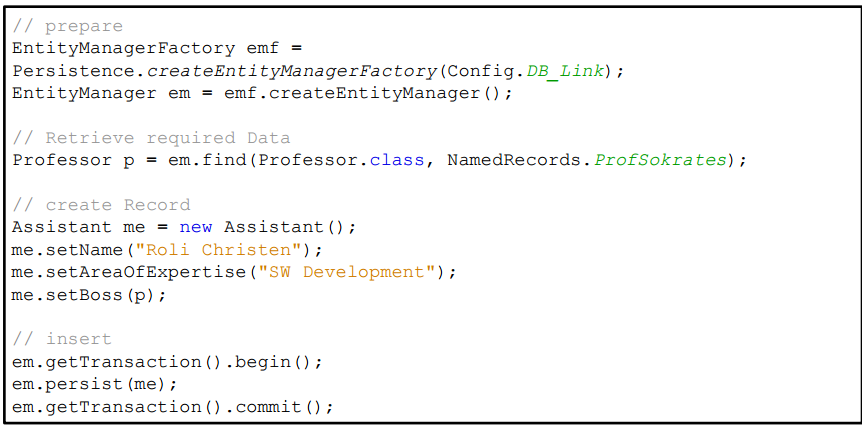
\includegraphics[width=0.8\linewidth]{fig/sample-jpa-code}
\caption{Beispiel Code JPA}
\label{fig:sample-jpa-code}
\end{figure}

Nachfolgend einige JPA-Methoden und Pitfalls:
\begin{itemize}
	\item em.remove(Entity e): Löschen einer Entity.
	\item persist vs merge: Persist inserted oder updated ein Entity und macht diese managed. Merge inserted oder updated eine Entity und macht diese aber nicht managed!
	\item managed (attached) vs unmanaged (dettached): Falls man mit einem managed Entity arbeitet und ein Attribut Wert ändert, wird dies direkt auf der Datenbank aktualisiert. Bei den unmanaged ist dies nicht der Fall und man muss nachträglich noch persist bzw. merge aufrufen.
\end{itemize}

\subsection{JPQL}
Dient um die Objekte mit einer objektorientierten Sprache abzufragen (siehe Abbildung \ref{fig:sample-jpql-code}. Wenn man JPQL verwendet, besteht immer die Gefahr, dass der String (JPQL Code) falsch geschrieben wurde. Passiert natürlich mit sauberem Testing nicht :). Trotzdem kann uns der Compiler hier nicht helfen und haben Code, welcher erst zur Runtime sein wahres Gesicht zeigt. Eine Alternative ist der CriteriaBuilder, welcher voll-typisierte Abfragen ermöglicht. Dieser ermöglicht es, dass wir keine ungültigen Abfragen schreiben!! Aber dieser scheint nicht Teil dieses Moduls zu sein.

\begin{figure}[h!]
\centering
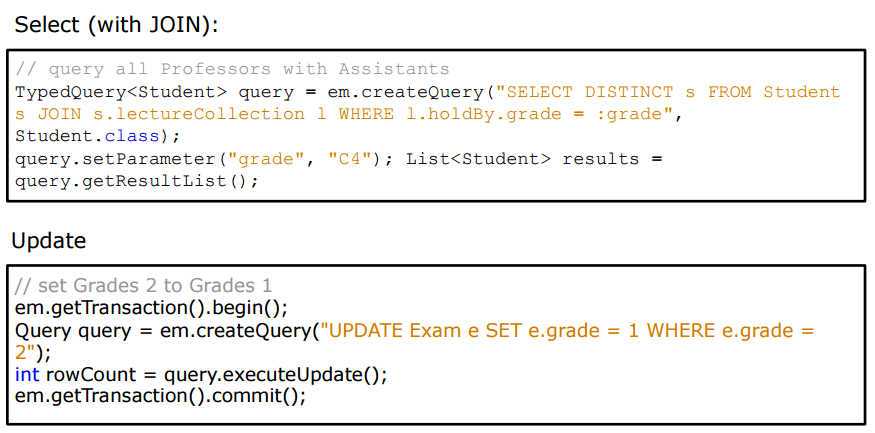
\includegraphics[width=0.8\linewidth]{fig/sample-jpql-code}
\caption{JPQL Code}
\label{fig:sample-jpql-code}
\end{figure}

\subsection{Caching}
Achtung der EntiyManager cached! Wenn ich die Liste aller Studenten eines Professors lade, anschliessend einen Student lösche und nochmals diesselbe Liste lade, können wieder dieseleben Entities daherkommen. Man kann die Liste mittels em.refresh(List<?> list) aktualisieren. Oder Den Cache des EM mittels evictAll() löschen. Oder das Entity manuell aus der Liste löschen oder Framework Features verwenden wie \emph{orphanRemoval=true}.







\end{document}